% In the previous chapter,
% we framed the task of answering a question $x$ on a table $w$
% as a semantic parsing task:
% generate a set $\zx$ of candidate logical forms,
% and then output $z \in \zx$ with the highest score.
% The goal is to predict a \emph{consistent} logical form;
% i.e., a logical form $z$ whose denotation
% matches the right answer $y$.

% While using patterns to guide search
% as explained in Chapter~\ref{chp:macro}
% increases the overall efficiency,
% performing search over the logical forms during training
% still poses two other fundamental issues.

So far,
we have been using the correct denotation (annotated answers)
as a distant supervision for training the semantic parser.
As argued in Chapter~\ref{chp:tables},
using distant supervision has several benefits.
Since the annotators do not have to learn the syntax of logical forms,
more annotations can be gathered more cheaply.
Furthermore, the annotation is independent of logical formalism,
meaning that we are free to choose any logical formalism
to attack the task.
Finally, more diverse types of questions can be gathered
since we do not limit the types of logical operations that
can be performed.

Despite these benefits,
training with denotation as supervision
requires running a search algorithm to find consistent logical forms
for parameter updates.
While doing so is fine in closed-domain settings,
% During training,
% the parser spends its time searching for logical forms
% by constructing them with deduction rules.
with the increased domain size (\Breadth)
and question complexity (\Depth),
it is increasingly
difficult to search over the space of logical forms
for two reasons:

\begin{figure}[tp]
\centering
\textsf{
\begin{tabular}{|c|c|c|c|c|} \hline
\textbf{Year} & \textbf{Venue} & \textbf{Position} & \textbf{Event} & \textbf{Time} \\ \hline
2001 & Hungary & 2nd & 400m & 47.12 \\
2003 & Finland & 1st & 400m & 46.69 \\
2005 & Germany & 11th & 400m & 46.62 \\
2007 & Thailand & 1st & relay & 182.05 \\
2008 & China & 7th & relay & 180.32 \\ \hline
\end{tabular}
}
\begin{tabular}{r@{\; }l}
$x$: & \nl{Where did the last 1st place finish occur?} \\
$y$: & Thailand \\
\end{tabular}
\\[0.5em]
%
\begin{tabular}{r@{\; }l} \toprule
\addlinespace

\multicolumn{2}{c}{\textbf{Consistent and semantically correct}} \\
\addlinespace

$z_1$: & {$\xOf{Venue}.\T{argmax}(\xHas{Position}.\T{1st}, \lambda r[\xOf{Index}.r])$} \\
\explainD{Among the rows with \emph{Position} = 1st, pick the one with maximum index and return its \emph{Venue}.} \\
\addlinespace

$z_2$: & {$\xOf{Venue}.\xHas{Index}.\T{max}(\xOf{Index}.\xHas{Position}.\T{1st})$} \\
\explainD{Find the maximum index of rows with \emph{Position} = 1st. Return the \emph{Venue} of the row with that index.} \\
\addlinespace

$z_3$: & {$\xOf{Venue}.\T{argmax}(\xHas{Position}.\xHas{Num}.\C{1}, \lambda r[\xOf{Date}.\xOf{Year}.r])$} \\
\explainD{Among the rows with \emph{Position} number 1, pick the one with the largest \emph{Year}. Return its \emph{Venue}.} \\
\addlinespace

\midrule
\addlinespace

\multicolumn{2}{c}{\textbf{Consistent but spurious}} \\
\addlinespace

$z_4$: & {$\xOf{Venue}.\T{argmax}(\xHas{Position}.\xHas{Num}.\C{1}, \lambda r[\xOf{Num}.\xOf{Time}.r])$} \\
\explainD{Among the rows with \emph{Position} number 1, pick the one with the largest \emph{Time}. Return its \emph{Venue}.} \\
\addlinespace

$z_5$: & {$\xOf{Venue}.\xHas{Year}.\xHas{Num}.\T{sub}(\xOf{Num}.\xOf{Year}.\T{argmax}(\T{allRows}, \lambda r[\xOf{Index}.r]), \C{1})$} \\
\explainD{Subtract 1 from the \emph{Year} in the last row, then return the \emph{Venue} of the row with that \emph{Year}.} \\
\addlinespace

\midrule
\addlinespace

\multicolumn{2}{c}{\textbf{Inconsistent}} \\
\addlinespace

$\tilde z$: & {$\xOf{Venue}.\T{argmin}(\xHas{Position}.\T{1st}, \lambda r[\xOf{Index}.r]) \qquad \to \deno{\tilde z}{w} = \set{\T{Finland}}$} \\
\explainD{Among the rows with \emph{Position} = 1st, pick the one with minimum index and return its \emph{Venue}.} \\
\addlinespace

\bottomrule
\end{tabular}
\caption[
Example of correct and spurious logical forms.
]{Six logical forms
generated from the question $x$.
The first five are \emph{consistent}:
they execute to the correct answer $y$.
Of those, \emph{semantically correct}
logical forms $z_1$, $z_2$, and $z_3$
are different ways to represent the semantics of $x$,
while \emph{spurious} logical forms $z_4$ and $z_5$
get the right answer $y$ for the wrong reasons.}
\label{fig:dpd-running}
\end{figure}

\begin{enumerate}
\item
\textbf{Exploding search space.}
the number of possible logical forms grows exponentially with
the size of logical forms.
In the previous chapters,
we use various techniques such as beam search,
deduction rule design,
pruning strategies,
and macro deduction rules
(Chapter~\ref{chp:macro})
to control the search space.
However, such techniques can prune away consistent
logical forms, which could slow down training.

\item
\textbf{Spurious logical forms.}
Spurious logical forms are logical forms that execute
to the right answer for a wrong reason.
For instance, the logical forms $z_1$, $z_2$, and $z_3$
in Figure~\ref{fig:dpd-running}
are \emph{semantically correct} as they follow what
the question $x$ asks;
however, $z_4$ and $z_5$ are \emph{spurious}:
they execute to the correct answer $\set{\T{Thailand}}$
but do not reflect what the question $x$ asks.
While increasing the search space
helps with coverage and generalization,
many spurious logical forms get generated.
Spurious logical forms provide deceptive signals during training.
For example, questions with the phrasing \nl{X or Y}
tend to have a lot of spurious logical forms,
and the model may not learn the correct construct $X \sqcup Y$
if it keeps updating toward spurious logical forms.
\end{enumerate}

As distant supervision is the root cause of the challenges above,
we propose to convert distant supervision into
\emph{direct supervision}.
% In other words,
% instead of running expensive search at training time
% to find consistent logical forms
% (and hoping that most of them are not spurious),
% we factor out the search process as a preprocessing step.
In other words,
we propose to
preprocess each example $(x, w, y)$ in the training data
by augmenting it with a set $\zsx$
of semantically correct logical forms.
We can then use $\zsx$
to train a semantic parser
that uses logical forms for supervision.
By factoring out the search process into a preprocessing step,
we can avoid running the expensive and potentially spurious
search process at training time,
thus sidestepping the two challenges outlined above.

Our approach for computing $\zsx$ from the given example
$(x, w, y)$ consists of two steps:
\begin{enumerate}
\item \textbf{Enumerate consistent logical forms.}
Given a question $x$, a table $w$, and a target denotation $y$,
compute a set $\zcx$ of logical forms consistent with
the denotation $y$.
To ensure the coverage of consistent logical forms
over an exponentially large search space of logical forms,
we propose \emph{dynamic programming on denotations} (DPD)
which uses the denotations of logical forms
to compress the search space to a manageable size.

\item \textbf{Filter out spurious logical forms.}
From $x$, $w$, $y$, and $\zcx$,
compute a subset $\zsx \subseteq \zcx$
of semantically correct logical forms.
As the denotation $y$ alone does not provide enough information
to detect spurious logical forms,
we instead turns to external signals from humans.
We propose \emph{fictitious tables}
as a framework to crowdsource signals for filtering
spurious logical forms.
\end{enumerate}

We will explain the two steps in the following sections,
and then wrap up with methods that can use the resulting
direct supervision to train the model.

\paragraph{Reference.}
The results described in this chapter have been published as
\cite{pasupat2016inferring}.
Reproducible experiments are hosted on the
CodaLab platform at
\begin{center}
\small
\url{https://worksheets.codalab.org/worksheets/0x47cc64d9c8ba4a878807c7c35bb22a42}.
\end{center}

\section{Enumerating consistent logical forms}
For a given example $(x, w, y)$,
our first step toward computing
semantically correct logical forms
is to generate the set $\zcx = \set{z \in \zx \mid \deno{z}{w} = y}$
of consistent logical forms.
We first reason why performing regular beam search
on the space of logical forms is intractable.
After that, we propose
\emph{dynamic programming on denotations} (DPD),
which performs search on the space of denotations instead.

\begin{table}[!p]\centering
\begin{tabular}{@{\;}lr@{ $\to$ }ll@{}} \toprule
\multicolumn{3}{c}{\textbf{Rule}} & \textbf{Semantics} \\ \midrule

\multicolumn{4}{c}{\textbf{\emph{Terminal Rules}}} \\

T1 &
$\C{TokenSpan}$ & $\C{Set}$ & $\mathrm{fuzzymatch}(s)$ \\
\explainC{cell or cell part fuzzily matching the text: \nl{chinese} $\to$ \T{China}} \\

T2 &
$\C{TokenSpan}$ & $\C{Set}$ & $\mathrm{value}(s)$ \\
\explainC{interpreted value: \nl{march 2015} $\to$ \C{2015-03-XX}} \\

T3 &
$\varnothing$ & $\C{Set}$ & $\T{allRows}$ \\

T4 &
$\varnothing$ & $\C{Set}$ & $\mathrm{closedClass}()$ \\
\explainC{entities from a column with few unique entities} \\
\explainC{e.g., \T{400m} or \T{relay} from the \emph{Event} column} \\

T5 &
$\varnothing$ & $\C{Rel}$ & $\mathrm{graphEdges}()$ \\
\explainC{\emph{any} graph edge: \T{Venue}, \T{Index}, \T{Next}, \T{Num2}, \dots} \\

T6 &
$\varnothing$ & $\C{Rel}$ & $\T{!=} \mid \T{<} \mid \T{<=} \mid \T{>} \mid \T{>=}$ \\

\midrule

\multicolumn{4}{c}{\textbf{\emph{Compositional Rules}}} \\

C1 &
$\C{Set} + \C{Rel}$ & $\C{Set}$ & $z_2.z_1 \mid \Mb{R}[z_2].z_1$ \\ 

C2 &
$\C{Set}$ & $\C{Set}$ & $A(z_1)$ \\
\explainC{$A \in \{\T{count}, \T{max}, \T{min}, \T{sum}, \T{avg}\}$} \\

C3 &
$\C{Set} + \C{Set}$ & $\C{Set}$ & $z_1 \sqcap z_2 \mid z_1 \sqcup z_2 \mid \T{sub}(z_1, z_2)$ \\
\explainC{subtraction is only allowed on numbers}  \\

\midrule

\multicolumn{4}{c}{\textbf{\emph{Compositional Rules with Maps}}} \\

\multicolumn{4}{c}{\textbf{Initialization}} \\

M1 &
$\C{Set}$ & $\C{Map}$ & $(z_1, x)$ \\
\explainC{identity map} \\

\multicolumn{4}{c}{\textbf{Operations on Map}} \\

M2 &
$\C{Map} + \C{Rel}$ & $\C{Map}$ & $(u_1, z_2.b_1) \mid (u_1, \Mb{R}[z_2].b_1)$ \\
\explainC{$(u_1, b_1)$ is the logical form of the \C{Map} argument; $z_2$ is the \C{Rel} argument} \\

M3 &
$\C{Map}$ & $\C{Map}$ & $(u_1, A(b_1))$ \\
\explainC{$A \in \{\T{count}, \T{max}, \T{min}, \T{sum}, \T{avg}\}$} \\

M4 &
$\C{Map} + \C{Set}$ & $\C{Map}$ & $(u_1, b_1 \sqcap z_2) \mid (u_1, b_1 \sqcup z_2) \mid (u_1, \T{sub}(b_1, z_2))$ \\
M5 &
$\C{Map} + \C{Map}$ & $\C{Map}$ & $(u_1, b_1 \sqcap b_2) \mid (u_1, b_1 \sqcup b_2) \mid (u_1, \T{sub}(b_1, b_2))$ \\
\explainC{Rule M5 is allowed only when $u_1 = u_2$} \\

\multicolumn{4}{c}{\textbf{Finalization}} \\

M6 &
$\C{Map}$ & $\C{Set}$ & $\T{argmin}(u_1, \lambda x[b_1]) \mid \T{argmax}(u_1, \lambda x[b_1])$ \\

\bottomrule

\end{tabular}
\caption[Generic deduction rules.]{
Our new set of generic deduction rules.
The logical form of the $i$-th argument is denoted by $z_i$
(or $(u_i, b_i)$ if the argument is a \C{Map}).
The set of final logical forms contains any logical form
with category \C{Set}.
}\label{tab:dpd-rules}
\end{table}


\subsection{Generic deduction rules}
In order to gain more coverage over possible logical forms,
we will use a collection of deduction rules
that is extremely more general than the one used in our floating parser.
Table~\ref{tab:dpd-rules}
shows the new deduction rules.
The differences from the original rules are as follows:

\begin{itemize}
\item
The categories are more general.
Instead of tying the categories to table constructs
such as cells and columns,
we use table-independent categories \C{Set}, \C{Rel}, and \C{Map}.
We also increase the generality of several
compositional rules.
For example, subtraction can now be applied on any two sets.

\item
To increase the recall of cell predicates,
we add the rule
$\varnothing \to \C{Set}[\Mr{closedClass}()]$,
which can generate any cell predicate
from a column with few unique cell contents.
For instance, if a column with header \nl{alive}
only contain \nl{yes} or \nl{no},
the question might say \nl{\dots is alive \dots}
or \nl{\dots is dead \dots} to refer to these cells.
Instead of relying on the $\Mr{fuzzymatch}$ function,
which will fail in this case,
we generate \T{Yes} and \T{No} from these two cells.
Our assumption here is that a cell from a column with a large number
of unique cell contents is usually referred to directly,
while a cell from a column with only a few possible values
could be mentioned in a more indirect way.

\item
The special \C{Map} category represents a partially
construct lambda that can be executed.
In the original set of deduction rules,
the lambda functions for \T{argmin} and \T{argmax}
are constructed independently from the set
they operates on, making them not executable in some cases.
For instance, the lambda $\lambda x.\T{count}(x)$
cannot be executed without the knowledge
without the knowledge of $x$.
\C{Map} addresses this problem by including
the domain that the lambda operates on.

A \C{Map} object is a tuple $(u, b)$
of a \emph{finite} set $u$ and a binary relation $b$.
Its denotation $\deno{(u, b)}{w}$ is
$(\deno{u}{w}, \deno{b}{w}')$
where the binary $\deno{b}{w}'$ is $\deno{b}{w}$
with the domain restricted to the set $\deno{u}{w}$.
For instance,
the logical form $\T{argmax}(\xHas{Position}.\T{1st}, \lambda r[\xOf{Index}.r])$ can be constructed
following the derivation tree in Figure~\ref{fig:dpd-parse-ex}.
\end{itemize}

\begin{figure}[t]
\centering
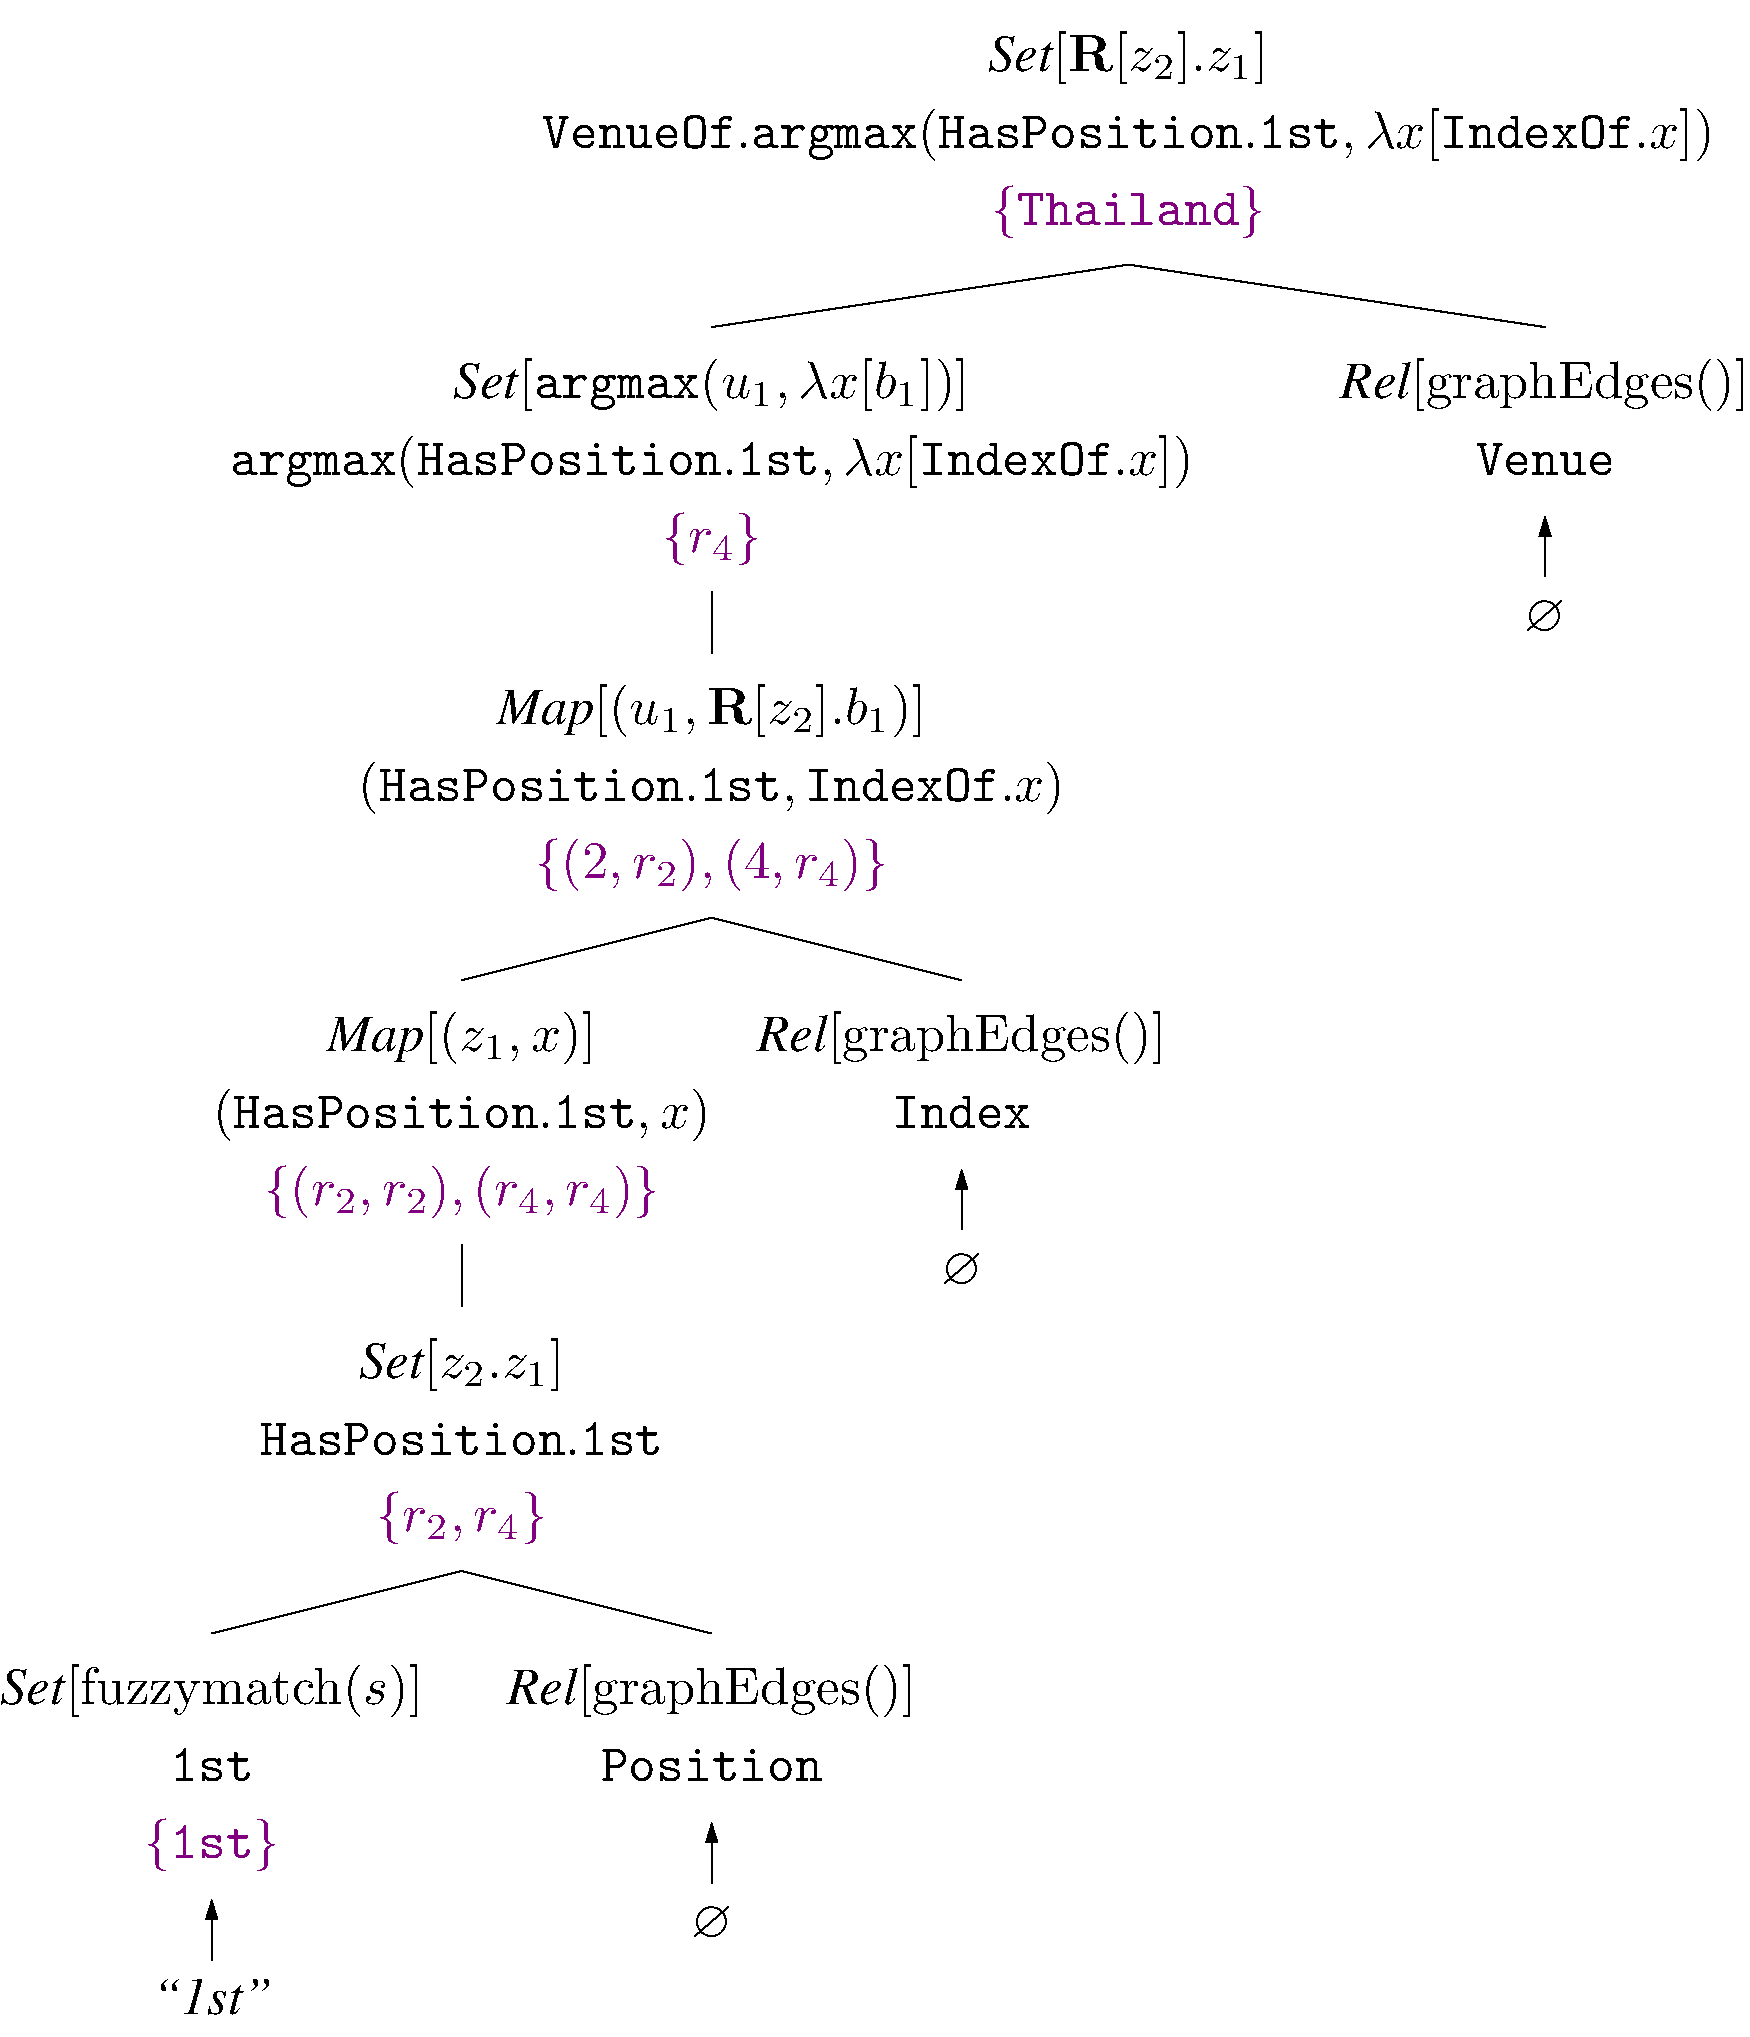
\includegraphics[scale=0.35]{sfig/parsetrees.slides/dpdParse.pdf}
\caption[Derivation tree of the running example under the \C{Map} construct.]
{A derivation tree for the utterance \runningEx
under our new set of deduction rules.
The denotations are shown in {\color[rgb]{.5, 0, .5}purple}.}
\label{fig:dpd-parse-ex}
\end{figure}

On top of the additional deduction rules,
we also introduce two new normalization edges to
the knowledge graph.
First, we use
\T{Num2} for the second number in the cell,
which usually denotes
a score of the opposing team or a measurement
in an alternative unit
(e.g., the cell node with text \nl{3--4} has
a \T{Num2} edge to atomic value \C{4}).
Second, we use
\T{Part} for items in a list
under a set of predefined list delimiters
(e.g., the cell with text
\nl{PC, Mac, Linux} has three \T{Part} edges
to \T{PC}, \T{Mac}, and \T{Linux}).
The $\Mr{fuzzymatch}$ method in Rule~T1
can generate these nodes representing cell parts
based on the utterance token spans.

\subsection{Dynamic programming on denotations}

From the deduction rules,
we could use our floating parser beam search to generate a set
of logical forms.
However, due to the generality of our deduction rules,
the set of of possible logical forms grows quickly
as the size of the logical forms increase.
As such, partial logical forms that are essential for
constructing the desired logical forms might
fall off the beam early on, resulting in an incomplete coverage.

\paragraph{Space of denotations.}
In order to reduce the search space,
our key observation is that while the number of logical forms
explodes quickly,
the number of \emph{distinct denotations}
of those logical forms grows at a much slower pace,
as multiple logical forms can share the same denotation.
For instance, the five consistent logical forms in
Figure~\ref{fig:dpd-running}
execute to the same denotation $\set{\T{Thailand}}$,
and variations in the arguments of logical operators
would create even more logical forms with that denotation.
% We can quantify this growth by plotting the
% number of distinct logical forms and their denotations
% as the logical form size increases.
% Figure~\ref{fig:lf-growth} shows that the space of logical forms
% explode much more quickly than the space of denotations.
% \todo{Details of this experiment, or maybe push to the experiments section}

Therefore, instead of directly enumerating logical forms,
we proposed \emph{dynamic programming on denotations} (DPD).
Inspired by similar methods in programming induction
\cite{lau03programming,liang10programs,gulwani2011automating,devlin2017robustfill},
the main idea is to group logical forms
with the same denotations together.
Instead of using cells $(c, s)$ of the floating parser
(where $c$ is the category and $s$ the the logical form size),
we perform dynamic programming on cells
$(c, s, d)$ where $d$ is a denotation.
For instance, the logical form
$\xHas{Position}.\T{1st}$
belongs to the cell $(\C{Set}, 1, \set{r_0, r_2})$.

One requirement for DPD to work
is that the deduction rules
must be \emph{denotationally invariant},
meaning that the denotation of the resulting logical form
must only depend on the denotations of its child
logical forms.
For example, a compositional rule 
with semantic function $g(z_1, z_2)$
is denotationally invariant if
\begin{equation}
\deno{z_1}{w} = \deno{z'_1}{w} \;\wedge\;
\deno{z_2}{w} = \deno{z'_2}{w} \implies
\deno{g(z_1, z_2)}{w} = \deno{g(z'_1, z'_2)}{w}
\end{equation}
As a counterexample, if the execution of $g(z_1, z_2)$
involves comparing the numbers of logical operators
in $z_1$ and $z_2$,
the rule is not denotationally invariant.

All deduction rules in Table~\ref{tab:dpd-rules}
are denotationally invariant.
As such, if any of our compositional rule
with semantic function $g(z_1, z_2)$
is applied on $z_1$ from cell $(c_1, s_1, d_1)$
and $z_2$ from cell $(c_2, s_2, d_2)$,
the resulting parse will belong to the same cell
$(c, s_1 + s_2 + 1, d)$ for some denotation $d$
regardless of which $z_1$ and $z_2$ are chosen.
The same conclusion applies for
compositional rules with only one child.
We will use this fact that logical forms in the same cell
are interchangeable to compress the search space
in the DPD algorithm.

\begin{figure}
\centering
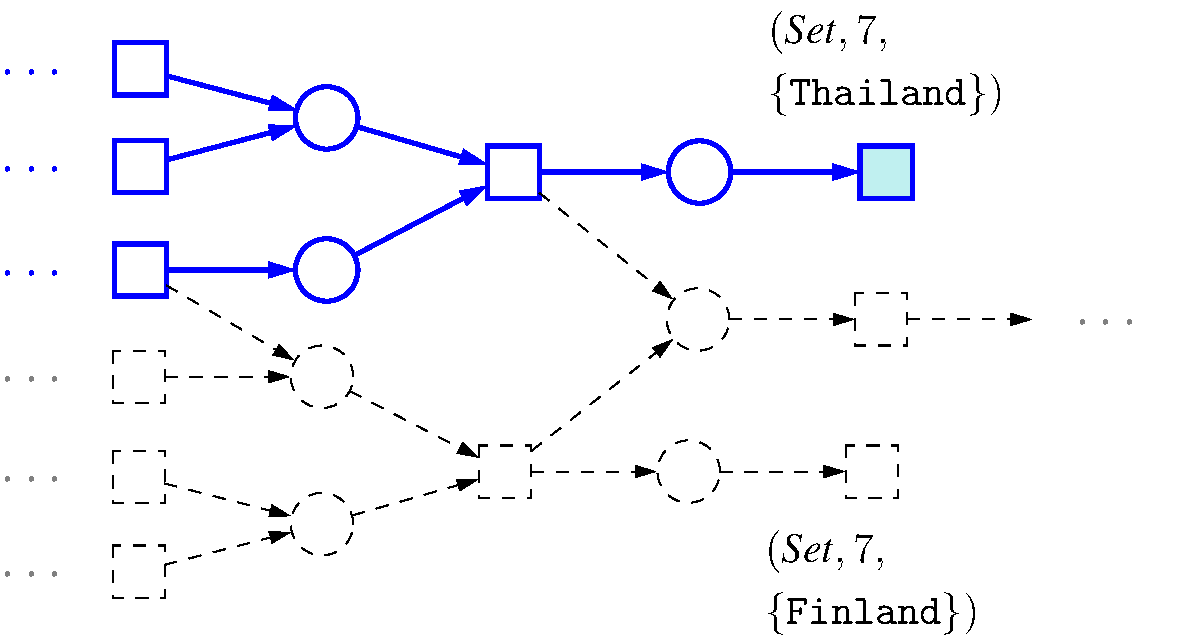
\includegraphics[scale=.4]{sfig/dpd.slides/dpdConcept.pdf}
\caption[Illustration of the DPD algorithm.]
{The first phase of DPD constructs
cells $(c,s,d)$ (square nodes)
using denotationally invariant semantic functions
(circle nodes).
The second phase enumerates all logical forms
along paths that lead to the correct
denotation $y$ ({\color{blue}solid lines}).}
\label{fig:dpd-figure}
\end{figure}

\paragraph{Algorithm.}
As illustrated in Figure~\ref{fig:dpd-figure},
the DPD algorithm consists of two phases.
The first phase finds the possible combinations of cells
$(c, s, d)$ that lead to the correct denotation $y$,
while the second phase enumerates the actual logical forms
belonging to the cells found in the first phase.

\begin{enumerate}
\item 
In the first phase,
we are only concerned about finding relevant cell combinations
and not the actual logical forms.
Therefore, any logical form that belong to a cell
could be used as an argument
of a deduction rule to construct further logical forms.
Thus, we ``collapse'' the logical forms
by keeping only at most one logical form per cell.
Subsequent logical forms generated for the same cell
are discarded,
but the combinations of children cells are recorded
for later backtracking.

After populating the cells up to some maximum size $s_\Mr{max}$,
we list all cells $(\C{Set}, s, y)$
with the correct denotation $y$,
and then note all possible cell-rule combinations
$(\Mr{cell}_1, \Mr{rule})$
or $(\Mr{cell}_1, \Mr{cell}_2, \Mr{rule})$
leading to those final cells,
including the combinations that yield discarded logical forms.

\item
The second phase retrieves the actual logical forms
by populating the cells $(c, s, d)$ with actual logical forms
using only the relevant cell-rule combinations
from the first phase.
Even though we are searching over the space of logical forms,
the elimination of irrelevant cell-rule combinations
effectively reduces the search space.
As our experiment in Section~\ref{sec:dpd-experiment} will show,
the number of cells needed to consider
is reduced by 98.7\%.
\end{enumerate}

\paragraph{Pruning.}
While denotations help us narrow down the search space,
there are a few cases where the search is still out of control.
We decide to sacrifice some generality
by introducing the following pruning procedures:

\begin{itemize}
\item We prune logical forms that are clearly redundant.
For instance, we prune any rule application that
does not change the denotation
(e.g., applying \T{max} on a set of size 1).
\item We restrict the union operation to between two cells
(e.g., $\T{Germany} \sqcup \T{Thailand}$)
since union rarely appears in other contexts.
\item We forbid the subtraction operation
when building a \C{Map}.
\item We do not allow \T{count} on a set of size 1.
This is the most restrictive heuristic since a small number
of questions require counting a set of size 1.
However, without this restriction, there are too many
logical forms that execute to $\set{1}$,
which can then be applied in other mostly irrelevant contexts
(e.g.,
selecting the first row with
$\xHas{Index}.\T{count}(z)$
where $\deno{\T{count}(z)}{w} = \set{1}$
will almost always be spurious.)
\end{itemize}

\subsection{Experiments} \label{sec:dpd-experiment}

\begin{figure}
\centering
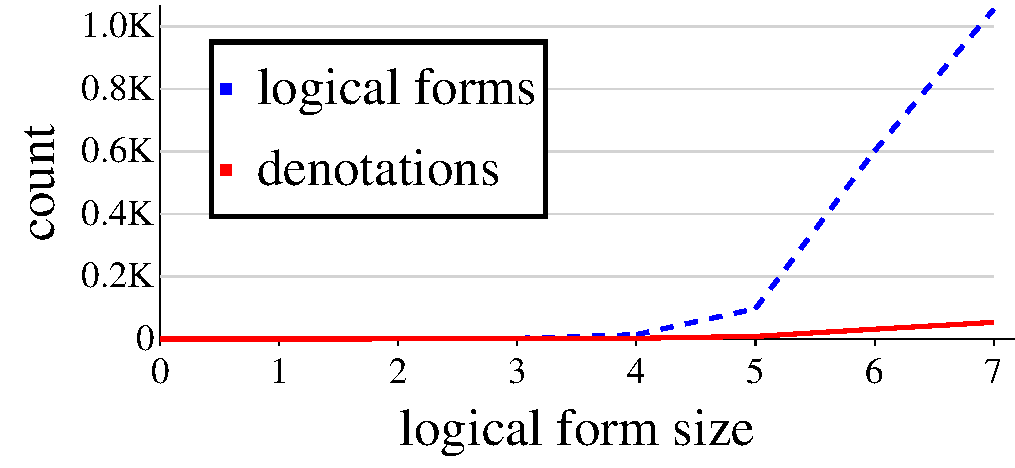
\includegraphics[scale=.4]{sfig/dpd.slides/exGrowth.pdf}
\caption[The space of denotations grows much more slowly than the space of logical forms]{The median of the number of
logical forms ({\color{blue}dashed})
and denotations ({\color{red}solid})
as the formula size increases.
The space of logical forms grows much more quickly
than the space of denotations.}
\label{fig:dpd-lf-growth}
\end{figure}

\begin{figure}[t]
\centering
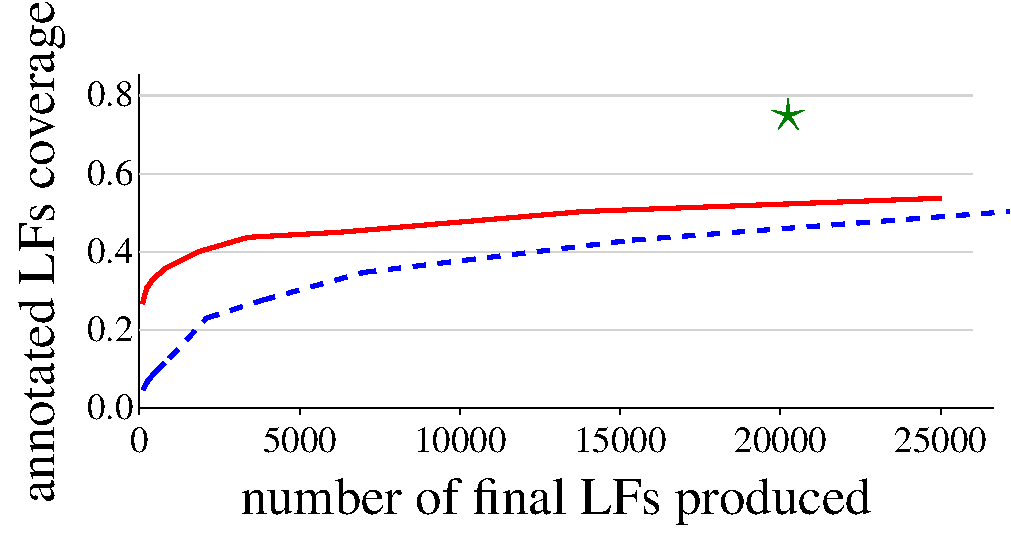
\includegraphics[scale=0.45]{sfig/dpd.slides/exFloat.pdf}
\caption[DPD has more coverage over the
annotated logical forms than beam search]{
The number of annotated logical forms
that can be generated by beam search,
both uninitialized ({\color{blue}dashed})
and initialized ({\color{red}solid}),
increases with the number of candidates generated
(controlled by the beam size),
but still lacks behind DPD ({\color{green!50!black}star}).}
\label{fig:dpd-results}
\end{figure}

% We use the training data of the \wtq dataset
% for our experiments.

\paragraph{Oracle.}
We manually annotate 300 training examples
from the \wtq dataset
with semantically logical forms if possible.
Among them, we successfully annotated 84\% of the examples,
which is a pretty good coverage since the crowd workers
who wrote the questions could have used the tables
in any way they wanted.
The remaining 16\% contains the types of reasoning
outside our setup.
Some of these include special table layouts,
answers that appear inside running texts or images
(instead of appearing as the whole cell
or a clearly demarcated part),
and questions that require common sense knowledge
(e.g., comparing \nl{Quarter-final} with \nl{Round of 16}
cannot be done by our \T{argmax}).

\paragraph{Search space.}
To demonstrate the savings gained by collapsing logical
forms with the same denotation together,
we plot the
number of distinct logical forms and their denotations
as the logical form size increases.
Figure~\ref{fig:dpd-lf-growth} shows that
the space of logical forms
explode much more quickly than the space of denotations.
Since the first phase of DPD operates
on the space of denotations,
the search is much more controlled than using beam search
over the space of logical forms.

Moreover,
DPD allows us to ignore a large number of irrelevant
partial logical forms before doing a fine-grained search
in the space of logical forms.
On average over all 14,152 training examples,
DPD generates approximately 25,000
consistent logical forms.
The first phase of DPD generates
approximately 153,000 cells $(c, s, d)$.
After filtering for the cell-rule combinations
that lead to the correct denotations,
only about 2,000 cells from 8,000 cell-rule combinations
remain, resulting in a 98.7\% reduction
of the number of cells we need to consider.

\paragraph{Coverage.}
To measure how well DPD enumerates consistent logical forms,
we consider the following experiment.
For each of the 300 training examples from earlier,
we run the DPD algorithm
to generate a set of consistent logical forms,
and then check if the annotated logical form is in the generated set.
We compare DPD against two baselines:
beam search with random parameters,
and beam search with parameters trained on the training data
of \wtq
using the method from Chapter~\ref{chp:parsing}.
The evaluation metric is coverage: the fraction of examples
where the annotated logical form is among the
generated logical forms.

Figure~\ref{fig:dpd-results}
plots the coverage against the number of logical forms
produced by the algorithms.
DPD successfully generates more annotated logical forms
(76\%)
than beam search
(53.7\%),
even when beam search is guided by the learned parameters.

\section{Filtering spurious logical forms}


\subsection{Fictitious tables}
After computing the set $\zcx$ of consistent logical forms,
the next step is to filter out spurious logical forms.
Unfortunately,
spurious logical forms and semantically correct ones
cannot be distinguished solely by considering their denotations
with respect to the table,
since the denotations will be identical by definition.
Instead, we use the following key observation:
if the same answer is asked on a different but similar tables
(e.g., having the same table schema but different cell contents),
semantically correct logical forms should give
a correct answer to the question in the new contexts,
while spurious logical forms will inevitably
fail in some contexts.
This is similar to how test cases are used to test programs:
a semantically correct program should correctly handle
the test inputs that follow the program's input specification,
while buggy programs may fail some test cases.

\begin{figure}[t]
\centering
\textsf{
\begin{tabular}{|c|c|c|c|c|} \hline
\textbf{Year} & \textbf{Venue} & \textbf{Position} & \textbf{Event} & \textbf{Time} \\ \hline
2001 & Hungary & 2nd & 400m & 47.12 \\
2003 & Finland & 1st & 400m & 46.69 \\
2005 & Germany & 11th & 400m & 46.62 \\
2007 & Thailand & 1st & relay & 182.05 \\
2008 & China & 7th & relay & 180.32 \\ \hline
\end{tabular}
}\\[.5em]$\downarrow$\\[.5em]
\textsf{
\begin{tabular}{|c|c|c|c|c|} \hline
\textbf{Year} & \textbf{Venue} & \textbf{Position} & \textbf{Event} & \textbf{Time} \\ \hline
2001 & Finland & 7th & relay & 46.62 \\
2003 & Germany & 1st & 400m & 180.32 \\
2005 & China & 1st & relay & 47.12 \\
2007 & Hungary & 7th & relay & 182.05 \\ \hline
\end{tabular}
}
\caption[
An example fictitious table.
]{
An example fictitious table generated from the table
in our running example.
}
\label{fig:fictitious-table}
\end{figure}

\paragraph{Generating fictitious tables.}
Based on the observation above,
we generate \emph{fictitious tables}
$w_1, w_2, \dots$ where each table $w_i$ is a slight
alteration of the original table $w$.
As illustrated in Figure~\ref{fig:fictitious-table},
the fictitious tables
maintain the original table schema (i.e., columns names),
but the cells in each column are re-sampled
from the pool of cell contents collected from
the original column.
The sampling process follows several guidelines:

\begin{itemize}
\item
If the cell contents of that column are originally all distinct,
sampling is done without replacement (i.e., the cells are permuted).
Otherwise, sampling is done with replacement.
\item
We want the cell predicates in the logical forms $z \in \zcx$
to be present in the fictitious table $w_i$.
To do so, any cell predicates that can be
generated by the terminal rules in Table~\ref{tab:dpd-rules}
need to appear in $w_i$.
\item
Columns where the cells are sorted usually have special semantics.
For instance, in Figure~\ref{fig:fictitious-table},
the latest event can be identified by performing \T{argmax}
on either the dates (literal semantics)
or the row indices (implied semantics: the rows are ordered
chronologically).
While one could argue that performing \T{argmax} on row indices
is spurious
under other contexts,
we will make a judgment call and decide that both approaches
are both semantically correct.
%\todo{Justify?}
As such, when constructing a fictitious table $w_i$,
we choose to keep sorted columns sorted
to preserves the implied semantics.
\end{itemize}

\begin{figure}[t]
\centering
\begin{tabular}{c|c|c|c|c@{}c@{ }l}
\multicolumn{1}{c}{} & \multicolumn{1}{c}{$w$} &
\multicolumn{1}{c}{$w_1$} & \multicolumn{1}{c}{$w_2$} & $\cdots$ \\ \cline{2-4}
$z_1$ & Thailand & China & Finland & $\cdots$ & \multirow{3}{*}{\Bigg\}} & \multirow{3}{*}{$q_1$} \\
$z_2$ & Thailand & China & Finland & $\cdots$ & \\ 
$z_3$ & Thailand & China & Finland & $\cdots$ & \\
$z_4$ & Thailand & Germany & China & $\cdots$ & \multirow{1}{*}{\}} & \multirow{1}{*}{$q_2$} \\
$z_5$ & Thailand & China & China & $\cdots$ & \multirow{2}{*}{\Big\}} & \multirow{2}{*}{$q_3$} \\
$z_6$ & Thailand & China & China & $\cdots$ & \\
$\vdots$ & $\vdots$ & $\vdots$ & $\vdots$ & \\ \cline{2-4}
\end{tabular}
\caption[Logical forms with the same denotation tuples are grouped into the same equivalence class]{
Consistent logical forms $z_i \in \zcx$
are executed on fictitious tables to get denotation tuples
$\deno{z_i}{W}$.
Logical forms with the same denotation tuple
are grouped into the same equivalence class $q_j$.}
\label{fig:equivalence-classes}
\end{figure}

\paragraph{Equivalence classes.}
Fictitious tables can help us identify logical forms
that are semantically equivalent
(under our assumption of implied column semantics above).
Let $W = (w_1, \dots, w_k)$ be a tuple of all possible
fictitious tables.
For a logical form $\zcx$, we define
its \emph{denotation tuple} as
$\deno{z}{W} = (\deno{z}{w_1}, \dots, \deno{z}{w_k})$.
We can now create equivalence classes $q$
of logical forms with the same denotation tuple,
which we will denote by $\deno{q}{W}$. 
For instance, in Figure~\ref{fig:equivalence-classes},
the logical forms $z_1$, $z_2$, and $z_3$ have the same
denotation across all fictitious tables,
and thus we group them into an equivalence class $q_1$.

When the question is unambiguous,
we expect at most one equivalence class
to contain semantically correct logical forms.

\subsection{Annotation}
To filter equivalence classes with spurious logical forms,
we acquire the correct answer to the question $x$
with respect to each fictitious table $w_i$ in $W$
from humans (e.g., via crowdsourcing).
We can filter out equivalence classes
whose denotation tuple does not match the annotated answers,
and then compile the rest into the collection $\zsx$
of semantically correct logical forms.

However, it is impractical and usually redundant
to collect the answer for all exponentially many fictitious tables.
So instead, we will approximate the process
by selecting some subset
$W' = (w'_1, \dots, w'_\ell)$ of $\ell$ fictitious tables
to be annotated with answers.

\paragraph{Choosing tables to annotate.}
We want to choose a subset $W'$ that can potentially
give us the most information about the correct equivalence class
as possible.
Let $\Mc{Q}$ be the collection of all equivalence classes.
Using the denotation tuples with respect to
$W' = (w'_1, \dots, w'_\ell)$,
we can divide $\Mc{Q}$ into partitions
\begin{equation}
F_t = \set{q \in \Mc{Q} : \deno{q}{W'} = t},
\end{equation}
where $t$ is a denotation tuple of length $\ell$.
For instance, in Figure~\ref{fig:equivalence-classes},
if $W'$ contains only $w_2$, then $q_2$ and $q_3$
will belong to the same partition $F_{(\T{China})}$.

Let the human-annotated answers form a tuple
$t^* = (y'_1, y'_2, \dots, y'_k)$.
Assuming that there is
at least one semantically correct logical form,
and that the human annotations are correct,
the answer tuple $t^*$ will identify exactly
one partition $F_{t^*}$.
This partition will include the
semantically correct equivalence class,
but can also include spurious equivalence classes
that are indistinguishable from the correct one based
on the fictitious tables in $W'$.
Our goal is to make the partitions as
\emph{small and numerous} as possible,
so that no matter what answer $t^*$ we get from humans,
the matched partition $F_{t^*}$ is likely to be small
(i.e., a large number of spurious logical forms are pruned away).

To make our objective more formal,
we choose $W'$ that maximizes
the \emph{expected information gained}
%(or equivalently, the reduction in entropy)
about the correct equivalence class given the annotation.
Define a random variable $Q \in \Mc{Q}$
representing the correct equivalence class,
and another random variable $T^*(W')$
for the annotation tuple
(which depends on our choice of $W'$).
Our objective is to find
\begin{equation}
W'
= \argmax_{W'} \nail{\HH[Q] - \HH[Q \mid T^*(W')]}
= \argmin_{W'}\;\HH[Q \mid T^*(W')],
\end{equation}
where the entropy terms $\HH[\cdot]$
measure the expected information,
and we want the entropy to reduce as much as possible
after observing the annotation.

We assume a uniform prior on the correct equivalence class $Q$:
\begin{equation}
p(Q = q) = \frac{1}{\card{\Mc{Q}}},
\end{equation}
and assume that the annotation is accurate with respect to $Q$:
\begin{equation}
p(T^*(W') = t \mid Q = q) = \cases{
1 &\cif{\deno{q}{W'} = t} \\
0 &\cotherw.}
\end{equation}
We can write
\begin{align}
p(T^*(W') = t, Q = q) &= \cases{
1/\card{\Mc{Q}} &\cif{\deno{q}{W'} = t} \\
0 &\cotherw} \\
p(T^*(W') = t) &= \frac{\card{F_t}}{\card{\Mc{Q}}}
\end{align}
(there are $\card{F_t}$ equivalence classes with
$\deno{q}{W'} = t$ due to the definition of $F_t$),
and therefore
\begin{align}
\HH[Q \mid T^*(W')]
&= -\sum_{q,t}p(q,t)\log \frac{p(q,t)}{p(t)} \\
&= -\sum_t \sum_{q; \deno{q}{W'} = t}
\frac{1}{\card{Q}}
\log \frac{1/\card{Q}}{\card{F_t}/\card{\Mc{Q}}} \\
&= \frac{1}{\card{\Mc{Q}}} \sum_t \card{F_t}\log \card{F_t}.
\label{eq:f-log-f}
\end{align}
We can search for $W'$ that minimizes
the term~(\ref{eq:f-log-f}) above.
This matches our original intuition
as the term is small
when the partitions $F_t$ are small and numerous.

In practice, we make a few more approximations:
\begin{itemize}
\item The full tuple $W$ of fictitious tables
is approximated as $k = 30$ randomly generated tables.
We then choose $W'$
by exhaustively searching over all possible combinations
of $\ell = 5$ fictitious tables.
\item We cannot guarantee that the annotations are all correct.
In our experiments, we propose several methods to trade off
accuracy with the amount of pruned spurious logical forms.
\end{itemize}

\subsection{Experiments}
We continue our investigation on the training examples
of the \wtq dataset.
The set $\zcx$ of consistent logical forms are computed
by the DPD algorithm.

\paragraph{Equivalence classes.}
Using 30 randomly generated fictitious tables,
we get an average of 1,237 equivalence classes per example.
To measure how well the true equivalence classes
(based on all possible fictitious tables)
are approximated by using on 30 fictitious tables,
we verify the equivalence classes against the ones
computed on 300 fictitious tables.
We found that only 5\% of the logical forms are separated
from the original equivalence classes.

\paragraph{Oracle annotation.}
For each of the 252 examples that were annotated
with semantically correct logical forms $z^*$
in Section~\ref{sec:dpd-experiment},
we use the denotation tuple $t^* = \deno{z^*}{W'}$
to simulate perfect human annotations.

By choosing a subset $W'$ of 5 fictitious tables that minimizes
our proposed objective function~(\ref{eq:f-log-f}),
we are able to prune out 98.7\%
of the spurious equivalence classes,
which equate to 98.3\% of spurious logical forms.
Additionally,
we were able to filter down to just one
equivalence class in 32.7\% of the examples,
and down to three classes in 51.3\% of the examples.
When more than one equivalence classes remain,
most of the time only one class will contain many
equivalent logical forms,
while other classes are small and contain
unusual logical forms such as the spurious $z_5$
in Figure~\ref{fig:dpd-running}.

If the 5 fictitious tables in $W'$ are chosen at random
instead of using our proposed method,
the number of examples that can be filtered down to
one and three classes reduce from 32.7\% to 22.6\% and
from 51.3\% to 36.5\%, respectively.

The average size of the equivalence class
containing the annotated logical form
is approximately 3,000
with a standard deviation of approximately 8,000.
As our logical formulation is very expressive,
there are many different logical forms
that equivalently represent the same semantics.

\paragraph{Human annotation.}
We now consider the answer tuple $t^*$
collected from crowdsourcing on Amazon Mechanical Turk.
We use 177 examples where at least two crowd workers
agree on the answer of the original table $w$.

The crowdsourced data is more susceptible to errors.
When using the answers on all 5 fictitious tables
to filter equivalence classes,
the entire set $\zcx$ of consistent logical forms
are pruned away in 11.3\% of the examples,
and the semantically correct equivalence class is pruned
in 9\% of the examples.
These errors are caused by annotation errors,
inconsistent data in the tables
(e.g., the \emph{Total} column
for sport medals
does not match the sum of the
\emph{Gold}, \emph{Silver}, and \emph{Bronze}
columns),
and different interpretation of the questions
on the fictitious tables.
For the remaining example,
we are able to filter out 92.1\% 
of spurious logical forms (which equates to
92.6\% of spurious equivalence classes).

To prevent semantically correct logical forms
from being pruned,
we relax our assumptions and keep any equivalence class
that disagree with the annotation $t^*$
in at most one fictitious tables.
The number of times the entire $\zcx$
is pruned out is reduced from
11.3\% to to 3\%,
but the number of spurious logical forms pruned
also decreases from 92.1\% to to 78\%.

\section{Using the generated logical forms}
The generated st $\zsx$ of semantically correct logical forms
can be used to train semantic parsers
that take logical forms as supervision.
For instance, \cite{krishnamurthy2017neural}
trains a neural semantic parser
by maximizing the log-probability of generating
100 shortest logical forms from $\zsx$.
By using the list $\zsx$,
the model does not need to perform search
during training.
Their single model achieves a test accuracy of 43.3\%,
while the ensemble model achieves an accuracy of 45.9\% .

Filtering spurious logical forms with fictitious tables
also turns out to be crucial.
When the model in \citet{krishnamurthy2017neural}
is trained on the set $\zcx$ of consistent logical forms
generated by DPD instead of the filtered $\zsx$,
the accuracy of the single model drops from 43.3\% to 36.3\%
\cite{mudrakarta2018it}.

\section{Related work and discussion}

\paragraph{Types of supervision for semantic parsing.}
As stated in the related work chapter 
(Section~\ref{sec:rw-knowledge-based-qa}),
machine learning models for semantic parsers
were mainly trained with logical forms as supervision
\cite{tang01ilp,wong07synchronous,zettlemoyer07relaxed,jia2016recombination,dong2016logical,zhong2017seq2sql}.
The logical forms provide a clear and semantically correct
signal, but they are expensive to annotate,
and the logical formalism would prematurely restricts the types
of questions present in the dataset.
Furthermore, as \citet{kushman2013regex} argues,
the annotated logical forms might not be the one
that best align with the utterance among
the equivalent logical forms.

Learning a semantic parser from denotations
\cite{clarke10world,liang11thesis,berant2013freebase}
was mainly motivated by the easiness of acquiring
annotated data.
However, for a broader domains and complex questions,
searching for semantically correct logical forms
become more difficult.
Some work tries to sidestep search,
such as by representing the process for computing answers
as continuous vectors instead of discrete symbols \cite{yin2016neural,neelakantan2016neural}.
% Others inject prior domain knowledge
% to bias the model toward semantically correct interpretations
% \citex.
Our work provides a general solution by converting
the distant supervision into direct supervision,
which opens the door for the large class of models that use
logical forms as supervision.

Previous works also considered other types
of supervision.
Without annotated logical forms or denotations,
GUSP \cite{poon2013gusp}
learns to translate dependency parses into semantic parse
by encouraging the result to be consistent with
the database schema.
\citet{krishnamurthy2012weakly} and
\citet{reddy2014large} encourage agreement
between the semantic parse and some other structure
(syntactic parse or semantic graph)
derived from the same declarative sentence.
Several previous works use interactive data,
such as dialog sessions or user feedback,
as a weak signal for interpreting the previous utterance
\cite{artzi11conversations,iyer2017neural,labutov2018learning}.

\paragraph{Test-driven program synthesis.}
The process of finding logical forms consistent
with the denotation is closely related
to test-driven program synthesis in the
programming language community.
The goal of program synthesis is to generate a program
that satisfies some specification,
such an input-output pairs.
Previous work has devised a similar idea
of dynamic programming on denotations
on more restricted spaces of programs
\cite{lau03traces,liang10programs,feser2015synthesizing,yaghmazadeh2016hierarchy},
When the program predicates are invertible,
such as in string manipulation
\cite{gulwani2011automating, parisotto2017sql, devlin2017robustfill},
the search can be made even more efficient.
More recently, \citet{wang2017program}
applies a similar technique to DPD on program synthesis,
but goes a step further to collapse
denotations of the same classes together
as another layer of abstraction.
However, doing so requires a bit more machinery
during unpacking to search over
logical forms.

\paragraph{Limitations of DPD.}
Dynamic programming on denotations depends on two assumptions
about the search space.
First, the number of unique denotations must be low
to prevent the number of cells in Phase 1 from exploding.
This means some logical form patterns, such as
arbitrary unions or subtraction between \C{Set}s or \C{Map}s,
cannot be handled effectively.
Luckily, such patterns do not occur often in the distribution
of natural questions.
Second, the number of unique logical forms that execute
to each denotation must be low; otherwise,
Phase 2 will have to search over too many logical form combinations.
One particular consequence is that \T{count} logical forms with
denotation $\{1\}$ will make the search space explode,
since many generated logical forms execute to sets of size 1.
This unfortunately reduces the coverage over correct logical forms
by approximately 2\%.

\paragraph{Test case generation.}
Our fictitious tables
functions similarly to test cases.
Previous work has considered generating
new test cases \cite{miller1990empirical},
but the goal there is to converge on a single program
rather than identifying a class of programs.

\paragraph{Avoiding spurious logical forms.}
When training with distant supervision,
the model can incorrectly updates toward spurious logical forms
found during search.
One way to avoid this without using additional annotations
is to ``hedge'' the updates:
in early training iterations,
perform updates toward consistent logical forms more equally
instead of proportionally to the probabilities assigned by the model.
This intuition, coupled with decoding strategies
that encourage more exploration,
can prevent the model from making bad updates toward spurious logical forms
\cite{guu2017bridging,misra2018policy}.

\section{Conclusion}
In this chapter,
we presented techniques for converting
distant supervision (denotations) into direct supervision
(logical forms).
Given the correct answer for a question
we efficiently enumerate logical forms consistent with the answer
using dynamic programming on denotations,
and then filter out spurious logical forms
with fictitious tables.
The resulting set of logical forms
can be used to train a directly supervised parser,
effectively sidestepping search problems during training.

The value of having logical forms as direct supervision
has been noted by \citet{yih2016value},
who used a labeling interface to annotate
questions in the \Sc{WebQuestions} dataset \cite{berant2013freebase}
with SPARQL queries.
Training with annotated queries as supervision
yields an increased accuracy,
and compared to the distantly supervised model,
the number of incorrect relations
%many errors that the model trained on denotations make
%are due to incorrect relations
learned through spurious logical forms
is decreased.
Our method of pre-computing logical forms
provides a more automatic method for annotating
examples with logical forms than the annotation interface.
While it still requires some human effort,
we do not require experts even when annotating complex questions.

Up to this chapter,
we have considered a new QA task that operates
on a high-\Breadth high-\Depth regime,
as well as algorithms based on semantic parsing 
to tackle the task.
The next chapter concludes our findings,
lists alternative QA methods in the literature
for solving our proposed task,
and provides several potential paths for future work.
